%  LaTeX support: latex@mdpi.com 
%  For support, please attach all files needed for compiling as well as the log file, and specify your operating system, LaTeX version, and LaTeX editor.

%=================================================================
\documentclass[entropy,article,submit,pdftex,moreauthors]{Definitions/mdpi} 

%=================================================================
% MDPI internal commands - do not modify
\firstpage{1} 
\makeatletter 
\setcounter{page}{\@firstpage} 
\makeatother
\pubvolume{1}
\issuenum{1}
\articlenumber{0}
\pubyear{2025}
\copyrightyear{2025}
%\externaleditor{Academic Editor: Firstname Lastname}
\datereceived{ } 
\daterevised{ } % Comment out if no revised date
\dateaccepted{ } 
\datepublished{ } 
%\datecorrected{} % For corrected papers: "Corrected: XXX" date in the original paper.
%\dateretracted{} % For corrected papers: "Retracted: XXX" date in the original paper.
\hreflink{https://doi.org/} % If needed use \linebreak
%\doinum{}
%\pdfoutput=1 % Uncommented for upload to arXiv.org
%\CorrStatement{yes}  % For updates


%=================================================================
% Add packages and commands here. The following packages are loaded in our class file: fontenc, inputenc, calc, indentfirst, fancyhdr, graphicx, epstopdf, lastpage, ifthen, float, amsmath, amssymb, lineno, setspace, enumitem, mathpazo, booktabs, titlesec, etoolbox, tabto, xcolor, colortbl, soul, multirow, microtype, tikz, totcount, changepage, attrib, upgreek, array, tabularx, pbox, ragged2e, tocloft, marginnote, marginfix, enotez, amsthm, natbib, hyperref, cleveref, scrextend, url, geometry, newfloat, caption, draftwatermark, seqsplit
% cleveref: load \crefname definitions after \begin{document}

%=================================================================
% Please use the following mathematics environments: Theorem, Lemma, Corollary, Proposition, Characterization, Property, Problem, Example, ExamplesandDefinitions, Hypothesis, Remark, Definition, Notation, Assumption
%% For proofs, please use the proof environment (the amsthm package is loaded by the MDPI class).

%=================================================================
% Full title of the paper (Capitalized)
\Title{Information Evolution by Bayesian Assembly}

% MDPI internal command: Title for citation in the left column
\TitleCitation{Information Evolution by Bayesian Assembly}

% Author Orchid ID: enter ID or remove command
\newcommand{\orcidauthorA}{0009-0007-7122-0317} % Add \orcidA{} behind the author's name

% Authors, for the paper (add full first names)
\Author{Dan Adler $^{1}$\orcidA{}}

%\longauthorlist{no}

% MDPI internal command: Authors, for metadata in PDF
\AuthorNames{Dan Adler}

% Affiliations / Addresses (Add [1] after \address if there is only one affiliation.)
\address{%
$^{1}$ \quad dan@danadler.com}

%\simplesumm{} % Simple summary

%\conference{} % An extended version of a conference paper

% Abstract (Do not insert blank lines, i.e. \\) 
\abstract{The emergence of complexity and information is a fundamental question spanning disciplines from physics to biology and computation. While traditional approaches describe information as an emergent property, they leave unresolved how it arises dynamically from purely abiotic processes. This paper presents Bayesian Assembly (BA) systems, an abstract framework that models the evolution of patterns through probabilistic interactions and stability-driven selection. By abstracting away specific physical laws, these systems demonstrate a universal mechanism for generating order and information. BA systems evolve patterns over successive generations, with selection pressures favoring stable configurations that persist and interact more frequently. These dynamics have the potential to encode logic, computational rules, and, under certain conditions, self-replicating behaviors, thereby offering a conceptual pathway to better understand the transition from abiotic to biotic evolution. However, substantial work remains to demonstrate these principles in realistic prebiotic scenarios or computational analogs. The framework also highlights the interplay between top-down and bottom-up causality, illustrating how emergent patterns recursively influence their formation while being shaped by local interactions. This study offers a computationally realizable pathway that may help bridge randomness and complexity. Further empirical validation and more detailed modeling are needed to confirm and refine these suggestions.
}

% Keywords
\keyword{Assembly Theory; Abiotic evolution; Emergent complexity; Information dynamics; Top-down causality; Bottom-up causality; Bayesian updating; Entropy reduction; Probabilistic interactions; Computational emergence; Prebiotic systems}


\graphicspath{{images/}}

%%%%%%%%%%%%%%%%%%%%%%%%%%%%%%%%%%%%%%%%%%
\begin{document}
%%%%%%%%%%%%%%%%%%%%%%%%%%%%%%%%%%%%%%%%%%

% The order of the section titles is different for some journals. Please refer to the "Instructions for Authors” on the journal homepage.

\section{Introduction}

The study of evolution, complexity, and information has been a cornerstone of multiple scientific disciplines that bridge physics, biology, and computation. Foundational works such as Schrödinger's \textit{What is Life?} \cite{schrodinger1944life} posed fundamental questions about how order emerges from disorder, inspiring theoretical explorations of how physical laws govern the emergence of biological systems. Tegmark's \textit{Mathematical Universe Hypothesis} \cite{tegmark2008mathematical} posits that the universe itself is a mathematical structure, where physical phenomena are manifestations of abstract mathematical rules. These works frame the question of complexity, but leave the mechanisms of emergence unaddressed.

In the realm of evolutionary dynamics, Fisher \cite{fisher1930genetical} and Nowak \cite{nowak2006evolutionary} provide mathematical models that describe the mechanisms of replication, mutation, and selection. Although these models illuminate the principles of biological evolution, they assume the existence of self-replicating, mutating entities and do not delve into how such entities might arise from purely abiotic processes. Similarly, Wheeler's concept of "It from Bit" \cite{wheeler1990itbit} intriguingly suggests that information underpins the physical world, but it lacks a concrete mechanism for how information structures form and evolve.

Dennis Noble's work on top-down causality \cite{noble2012causality} emphasizes the role of systems-level behavior in determining lower-level interactions. This perspective challenges reductionist paradigms, but does not address how such systems might emerge from simpler abiotic conditions. On the computational side, Seth Lloyd’s concept of the universe as a quantum computer \cite{lloyd2006programming} provides a framework for understanding the universe as a computational entity but leaves open the question of how specific computational rules or patterns arise.

Algorithmic complexity \cite{kolmogorov1965complexity} \cite{chaitin1977algorithmic} \cite{solomonoff1964formal} and Shannon’s information theory \cite{shannon1948mathematical} provide powerful tools to quantify information and complexity, but do not explain how information is created or evolves within physical systems. These frameworks focus on static measures of complexity, often missing the dynamic interplay between interactions and selection that drives the formation of ordered structures.

This paper introduces Bayesian Assembly (BA) systems which offer an abstract model for the emergence of complexity and information. Unlike prior work tied to physical systems or abstract concepts without implementation pathways, BA systems provide a plausible mechanism for how stable patterns might arise, evolve, and persist based solely on probabilistic interactions.

Constructor Theory \cite{deutsch2013constructor} provides a foundational framework for understanding physical laws in terms of counterfactuals—statements about which transformations are possible or impossible. This perspective shifts the focus from dynamical laws to the principles governing what can be constructed or maintained by physical systems, offering profound insights into how patterns emerge and persist. While Constructor Theory captures the essence of counterfactual properties, it does not explicitly address the generational dynamics through which such patterns evolve and are selected over time.

Recent developments in Assembly Theory (AT) \cite{walker2023nature} complement this by providing a quantitative framework for complexity, introducing the assembly index as a measure of the minimal number of recursive steps required to construct an object from basic building blocks. AT emphasizes how physical and historical constraints shape the combinatorial explosion of possibilities, offering a retrospective view of selection. However, while AT identifies selection as central to the emergence of complexity, it does not model the dynamic processes through which selection unfolds in real time.

Kauffman’s Theory of Adjacent Possible (TAP) emphasizes the combinatorial growth of adjacent possible configurations and introduces a quantitative measure for the rate of discovery within an expanding state space \cite{kauffman2024tap}. In contrast, Bayesian Assembly (BA) systems focus explicitly on how stability-driven selection governs the persistence and evolution of patterns, providing a dynamic probabilistic framework that complements and extends the more combinatorial perspective of TAP.

More elaborate chemical modeling systems, such as Mass Action Kinetics (MAK) \cite{TuranyiTomlin2014}, Chemical Reaction Network Theory (CRNT) \cite{feinberg1987chemical}, and the stochastic framework introduced by \cite{arxiv:q-bio0501016}, provide detailed, quantitative descriptions of reaction dynamics, often incorporating conservation laws and equilibrium states. These systems excel at modeling well-defined reaction pathways, particularly in chemical and biochemical systems, but they typically require predefined reaction sets and fail to explore open-ended generativity. Tononi's integrated information theory (IIT) \cite{tononi2008phi} offers a different perspective by quantifying the complexity of neural and information systems through measures like $\Phi$, focusing on the integration and differentiation of information. Despite their strengths, these frameworks do not explicitly isolate selection as an emergent mechanism in the evolution of information.

Bayesian Assembly (BA) systems distinguish themselves by their narrow focus on stability as the central determinant of pattern persistence. Stability is simulated by associating different lifetimes with concatenated patterns, capturing the essential dynamics of selection without invoking detailed physical or chemical laws. This approach allows BA systems to isolate and model selection as the driving mechanism of information evolution. The term "Bayesian" reflects the iterative updating of probabilities for each pattern based on prior abundances and interactions. By emphasizing stability-driven selection in evolving state spaces, BA systems provide a dynamic and generative framework for studying how patterns are created, maintained, and ultimately evolve into complex configurations, complementing existing approaches while filling a crucial gap in our understanding of information evolution.

\section{BA System Fundamentals}

We define Bayesian Assembly (BA) Systems as follows: a population of base elements \( A, B, C, \dots \) capable of forming compounds through local interactions of unspecified forces. Compounds are represented as concatenations of base elements and other compounds, thus they can be repetitive and recursive. The elements could exist in our physical universe, or in an abstract universe. The stability of compounds is an abstraction that determines only one thing: how many generations they will persist. For example, if compound AAB has a stability of 10 then it will persist for 10 generations and then disappear. In contrast to bidirectional models like MAK, where dissipation of patterns is modeled explicitly, BA systems just allow the patterns to disappear. Since we do not constrain the interactions themselves in any way, compounds that have a stability of 0 may get created and destroyed in the same generation, which simulates impossible interactions. We allow the base elements to regenerate at a constant rate in every generation. This ensures a continuous influx of resources, preventing stagnation and enabling sustained exploration of the state space. This assumption mirrors the continuous flow stirred tank reactor (CFSTR) methodology commonly employed in chemical reaction modeling, where reactants are replenished at a constant rate to maintain steady-state conditions \cite{fogler1999chemical}. The analogy highlights the foundational role of resource replenishment in both theoretical and experimental systems for exploring dynamic behaviors and emergent patterns.

\begin{figure}[htp]
    \centering
    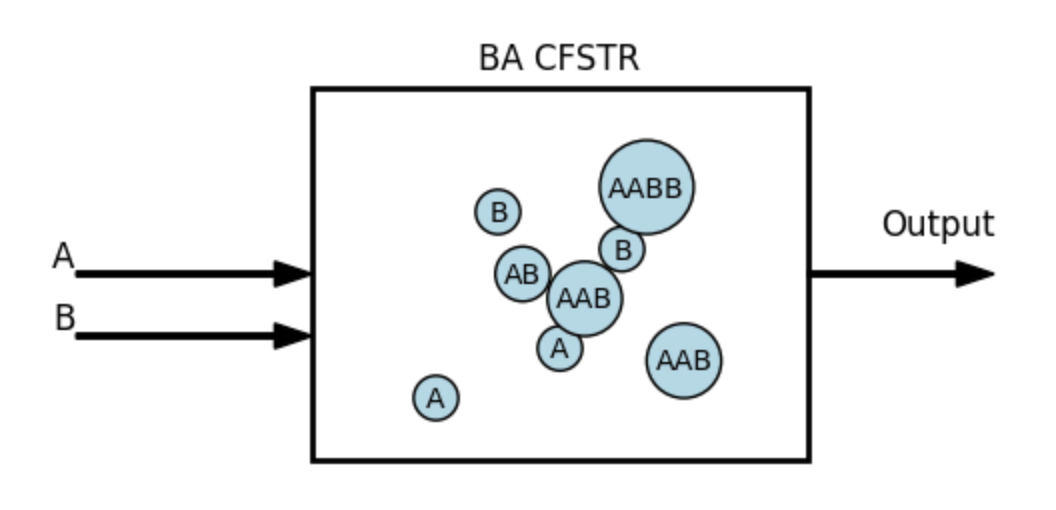
\includegraphics[height=4cm]{ba_cfstr}
    \caption{BA clocked equivalent of a Continuous Flow Stirred Tank Reactor (CFSTR)}
    \label{fig:ba_cfstr}
\end{figure}

Selection emerges naturally through the interplay of stability and probabilistic interactions. Consider a simple BA system starting with a few instances of base elements \( A \) and \( B \). The pattern \( AB \) has a lifetime of 10 generations, while \( ABAB \) has a lifetime of 50 generations, and all other compounds degrade instantly with a lifetime of 0. After the first generation, the system produces combinations such as \( AA \), \( BB \), and \( AB \). Since \( AA \) and \( BB \) are unstable, they are eliminated, leaving \( A \), \( B \), and \( AB \). In subsequent generations, new unstable patterns may appear transiently, but \( AB \) persists due to its longer lifetime. Over time, the population of \( AB \) increases probabilistically, as multiple instances of \( AB \) are likely to form, increasing the likelihood of forming \( ABAB \). This dynamic reflects a form of roulette wheel selection \cite{goldberg1989genetic} \cite{holland1975adaptation}, where the stability-driven persistence of \( AB \) amplifies its probability of interaction. The emergent pattern \( ABAB \) represents a higher-order configuration, demonstrating how selection, grounded in differential stability, shapes the system's evolutionary pathways. The mechanism relies on the stability-induced bias in interaction probabilities, ensuring that patterns with greater persistence are favored, enabling the accumulation of complexity over successive generations.

The following simulation shows a different BA system with a population of 3 elements: {A, B, C}. Assume B-compounds are more stable than those without B. Thus patterns like BB, AB, BC, ABC, have a higher stability than AC or A or C. Therefore, B compounds will persist for multiple generations, while the others will quickly dissipate. The more stable B-compounds will interact more frequently due to their relative frequency, even without replication or inheritance. A snapshot of the simulation is shown in Figure \ref{fig:pat_1}.

\begin{figure}[htp]
    \centering
    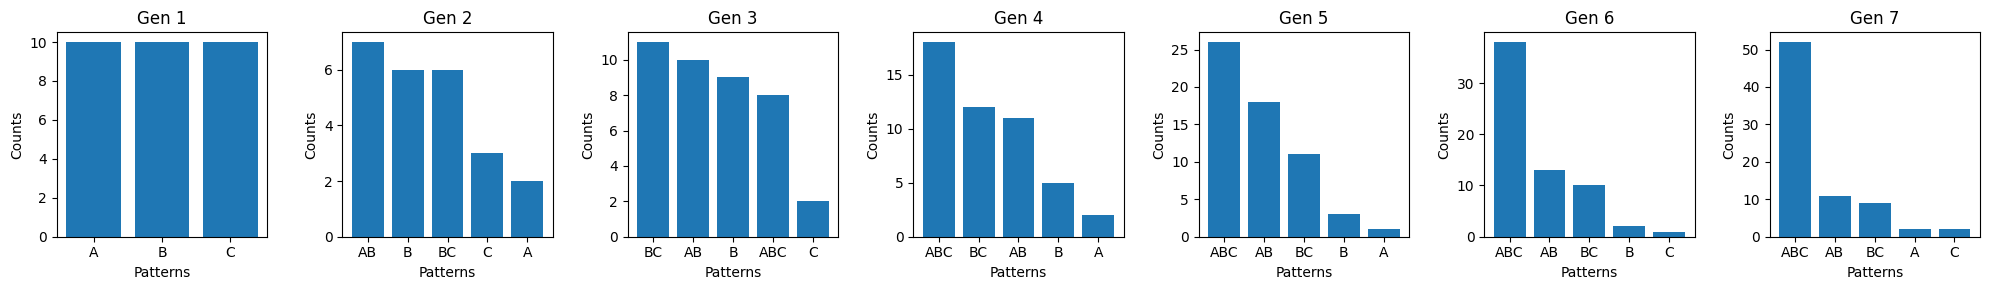
\includegraphics[width=13cm]{pat_1}
    \caption{BA System population evolution simulation}
    \label{fig:pat_1}
\end{figure}

Where is Maxwell's demon \cite{leff2002maxwell} hiding in this example, driving it towards a low-entropy state? As we saw, the answer lies in the roulette wheel. Compounds that persist longer have more chances to interact. As their frequency in the population grows, their chances to interact grow even more. In Evolutionary Dynamics, this is called fitness-proportionate selection \cite{back1996evolutionary} or roulette wheel selection \cite{goldberg1989genetic} \cite{holland1975adaptation}.

\section{Dual Probability Distributions Governing BA Systems}

BA systems can be effectively described by two interdependent probability distributions: the \textbf{population distribution}, which represents the relative abundance of patterns in the system, and the \textbf{stability distribution}, which quantifies the stable lifetime of successful compounds. The population distribution reflects the probabilities of patterns at any given generation \( t \). Let \( P_t(p) \) represent the probability of pattern \( p \) in the population at time \( t \):
\[
P_t(p) = \frac{N_t(p)}{\sum_{q \in P} N_t(q)}
\]
where \( N_t(p) \) is the absolute count of pattern \( p \) in the population at time \( t \), and \( \sum_{q \in P} N_t(q) \) is the total population size at time \( t \), ensuring normalization (\( \sum_{p \in P} P_t(p) = 1 \)). The population distribution evolves over generations as patterns interact and new stable configurations emerge. As patterns with higher stability and frequent interactions become more prominent in the population, the population distribution evolves to reflect the history of past interactions and selection pressures.

The stability distribution \( S(p) \) represents the persistence or longevity of the individual pattern \( p \) in the system, defined as the expected lifetime or persistence of \( p \) over generations. Stability is a measure of how long a pattern remains viable before it dissipates or is replaced, reflecting physical properties such as energy barriers, bond strengths, environmental effects, and resistance to degradation.

Stability influences the dynamics of the system by determining how long a pattern persists to participate in future interactions. Patterns with higher stability values \( S(p) \) are more likely to accumulate over generations, increasing their representation in the population and increasing the likelihood of forming new patterns. This persistence-driven selection creates a feedback loop, where stable patterns dominate the system dynamics, guiding the evolution of complexity. 

In simulations of real-world scenarios, the values of \(S(p)\) would reflect the underlying physical, chemical, or even economic or social principles. In a chemical context, for example, these stability factors might be derived from binding energies, reaction rate constants, or free energies of formation. In an economic model, they could represent relative cost efficiencies or market resilience. In each case, \(S(p)\) encodes the notion of persistence in the relevant domain: the likelihood that a given compound, pattern, or agent survives long enough to interact and persist into the next generation. Unlike the population distribution, which evolves dynamically based on interactions, the stability distribution remains constant or changes only gradually. 

\subsection{Combined Role of Population and Stability Distributions}

Together, the population and stability distributions determine the dynamics of the system. The full probability expression for the distribution at the next generation, including the normalization denominator, is:
\begin{equation}
\label{eq:ba_update}
P_{t+1}(p)
\;=\;
\frac{\,P_{t}(p)\;\cdot\;S\!\bigl(p\bigr)\,}
     {\sum_{p'\,\in\,P}\;\Bigl[P_{t}\!\bigl(p'\bigr)\;\cdot\;S\!\bigl(p'\bigr)\Bigr]}
\end{equation}

Intuitively, multiplying $P(p)$ by $S(p)$ reflects two factors: the initial abundance (or likelihood) of the pattern, and its ability to persist over enough time (generations) to interact repeatedly. Since $S(p)$ is interpreted as the expected lifetime of the pattern, then having more time (counted in generations) to react or be selected naturally increases its representation in the next update. Meanwhile, a pattern's prior probability $P(p)$ captures how commonly it appears in the current generation. Both a high initial abundance and a long lifetime can boost a pattern's success in the subsequent generation. For simplicity, we now use the proportional form in our discrete analysis:
\begin{equation}
P_{t+1}(p) \;\propto\; P_t(p)\,\cdot\,S(p)
\end{equation}
Here, $S(p)$ represents the stable lifetime of pattern $p$. Multiplying $P_t(p)$ by $S(p)$ ensures that patterns with higher stability gain an advantage in subsequent generations, as they remain available for more interactions or persist longer. This update rule encapsulates the idea that a stable pattern is more likely to be ``selected'' over time. To quantify the system-wide impact of stability, we define an \emph{effective stability}:
\begin{equation}
S_{\mathrm{eff}} \;=\; \sum_{p \in P}\; P_t(p)\,\cdot\,S(p)
\end{equation}
which measures the average or global level of stability in the population. If the system becomes dominated by highly stable patterns, $S_{\mathrm{eff}}$ grows, increasing the overall rate at which such patterns are reinforced. Conversely, if less stable patterns predominate, $S_{\mathrm{eff}}$ is smaller, slowing the formation of ordered structures. In a continuous-time limit approximation, we can write
\begin{equation}
\frac{dP(p,t)}{dt} \;\propto\; P(p,t)\,\cdot\,S_{\mathrm{eff}}
\end{equation}
leading to an exponential solution of the form
\begin{equation}
P_t(p) \;\propto\; e^{S_{\mathrm{eff}}\,t}
\end{equation}
This exponential growth demonstrates how feedback from stable patterns accelerates the ordering process, continually reinforcing those patterns that remain viable. Entropy changes arise from two competing processes. On the one hand, random fluctuations broaden the distribution (increasing entropy) at a logarithmic rate. As in other diffusive or random-walk scenarios, the accessible state space grows sub-exponentially (e.g., proportional to $\sqrt{t}$), causing the associated entropy to accumulate at a rate proportional to $\ln(t)$:
\begin{equation}
\Delta H_{\text{random}} \;\propto\; \ln(t)
\end{equation}
whereas reinforcing stable patterns focuses the distribution (decreasing entropy) at an exponential rate:
\begin{equation}
\Delta H_{\text{stability}} \;\propto\; -\,e^{S_{\mathrm{eff}}\,t}
\end{equation}
If the stabilizing feedback outpaces random diffusion, the net result is a persistent reduction in entropy, guiding the system toward ordered, low-entropy configurations characteristic of Bayesian Assembly (BA) dynamics.

\section{Mixing Two BA Systems}

Mixing two independently evolved BA systems introduces a new dimension to their dynamics, where patterns and interactions from each system influence the other. This interaction results in the exchange of information, changes in entropy, and the potential emergence of novel patterns. 

Let two independently evolved BA systems represent populations of compounds from different base elements \( A, B, C, \dots \) and \( X, Y, Z, \dots \), respectively. Each system evolves independently on the basis of its population distribution and stability constraints. When the two systems are mixed, the patterns from both interact, allowing the formation of compounds in the cross-system (e.g., \( ABXX, BBYZ \)). Stability constraints extend to intersystem interactions. The joint system evolves on the basis of updated probabilities reflecting both within-system and cross-system interactions.

\begin{figure}[htp]
    \centering
    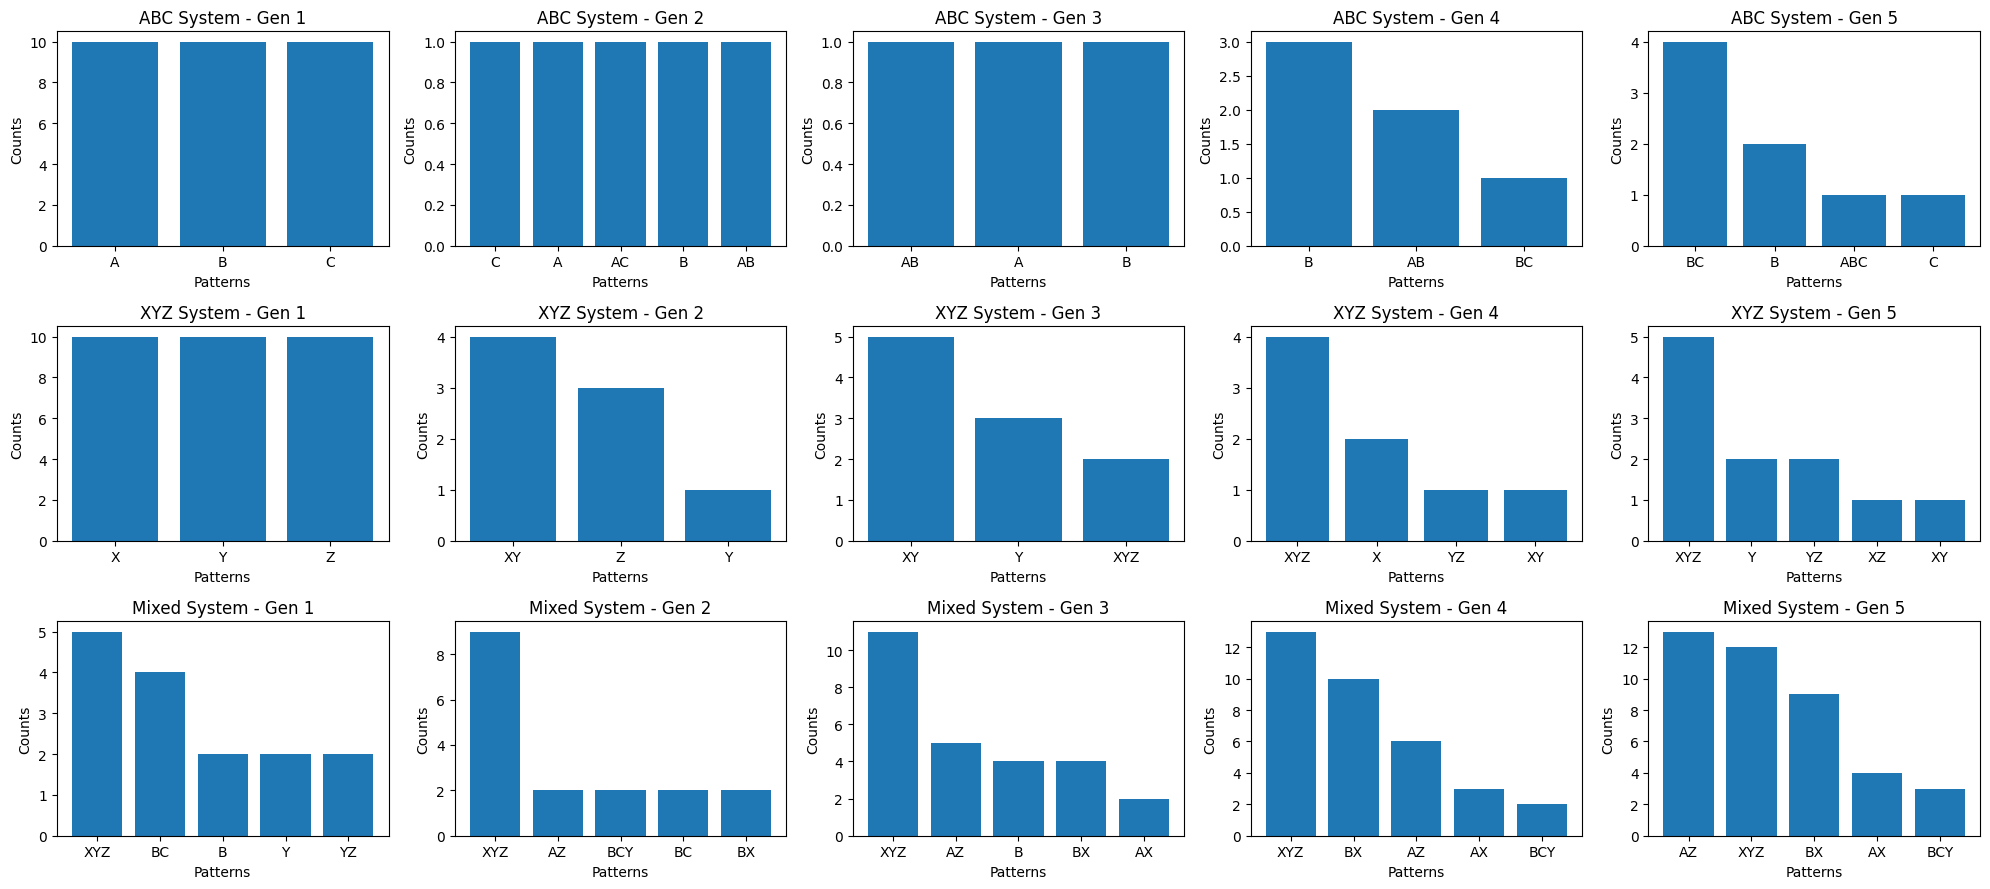
\includegraphics[width=13cm]{mixed_1}
    \caption{Mixing two evolved populations}
    \label{fig:mixed_1}
\end{figure}

In a continuous-flow stirred tank reactor (CFSTR) \cite{fogler1999chemical}, two different chemical feeds are mixed, producing a steady-state mixture. Once mixed, reactants from each feed can participate in cross-reactions, occasionally generating novel compounds (like AZ in the figure above) that surpass the stability of any compounds found in each feed. In a Bayesian Assembly (BA) analogy, new high-stability patterns proliferate over less stable alternatives. This explains how mixing can yield emergent compounds and reaction pathways that were inaccessible in isolation, driving a further entropy reduction.

\section{Bayesian Updating in BA Systems}

Kauffman's \emph{Theory of the Adjacent Possible} \cite{kauffman2000investigations} provides a useful conceptual backdrop for understanding how new states or patterns can emerge once existing states pave the way for them. In chemical and biological contexts, the ``adjacent possible'' refers to structures or configurations that become accessible only after certain precursors appear. In a Bayesian Assembly (BA) framework, such newly available patterns are those that can arise in generation $t+1$ but were beyond reach in generation $t$. The BA perspective adds a dynamic view of selection: it explicitly tracks how some of these emergent patterns persist and proliferate when they possess sufficient node stability. As we saw in Equation \ref{eq:ba_update} the BA generational update rule can be written as:
\begin{equation}
P_{t+1}(p) \;=\; 
\frac{\,P_t(p)\,\cdot\,S(p)\,}
     {\sum_{p' \in \mathcal{P}}\,P_t\!\bigl(p'\bigr)\,\cdot\,S\!\bigl(p'\bigr)},
\end{equation} 
This rule can be interpreted as a Bayesian evolutionary formula:

\begin{equation}
\text{New Probability (Posterior)}
\;=\;
\frac{\text{Old Probability (Prior)} \;\times\; \text{Stability (Likelihood)}}
     {\text{Normalization}}
\end{equation}
Stability plays the role of Likelihood in the Bayesian equation because it is a measure of the likelihood of the specific pattern to persist over time, thereby determining its chances of being selected to interact with other patterns in the next generations. This generational update, in turn, drives an evolutionary exploration of the adjacent possible: once a newly available pattern displays sufficiently high node stability, its probability can rise, thus reshaping the distribution of patterns in subsequent generations.

This interpretation of the evolving process aligns with the view of Bayesian probabilities as a hallmark of dynamical systems \cite{le2020equation}, where the distribution of each generation plays the role of the prior, and the posterior emerges as genuinely new distribution, rather than a subjective refinement of a single unknown distribution, allowing novel patterns and interactions to reshape the system over time. The distribution of compounds in each generation is determined by relative frequencies (reflecting a frequentist probability), while the transition to the next generation is driven by a Bayesian update process (reflecting an evolving Bayesian probability).

\section{Top-Down vs.\ Bottom-Up Dynamics in BA Systems}
\label{sec:topdown-bottomup}

Bayesian Assembly (BA) systems exhibit two complementary forms of causality, previously identified as \emph{bottom-up} and \emph{top-down}. From a bottom-up perspective, local probabilistic interactions drive the system's evolution by creating or dissolving patterns. These interactions are regulated by node stability and selection pressures, producing emergent order from initially simple building blocks. 

Once certain patterns become dominant, however, they exert a top-down influence on subsequent generations. These persistent, higher-level structures shape future interactions by catalyzing or constraining the formation of new patterns. Hence, BA systems do not merely accumulate complexity through local rules; they also incorporate feedback from emergent structures that guide (or ``select for'') new configurations. The presence of memory and evolutionary history in these feedback loops distinguishes BA systems from frameworks in which higher-level states simply describe aggregates without influencing the underlying microstates.

The contrast with traditional statistical mechanics is informative \cite{landau1980statistical}. In a typical statistical-mechanical setting, macrostates (e.g., temperature, pressure) characterize large-scale properties that reflect averages of microstates; they rarely feed back to alter the fundamental interaction rules among particles. By contrast, the dominant patterns in BA systems play a direct, causal role in shaping micro-level interactions. This effect renders BA systems capable of embedding history and specificity into the very process that generates new patterns, rather than relying on pre-defined energy distributions or equilibrium conditions.

Such an explicit interplay between bottom-up and top-down dynamics in BA systems suggests a broader principle for understanding complexity: emergent structures can become causal agents that direct further evolution of the system. This perspective helps explain the accumulation of novel order in contexts from prebiotic chemistry to computational networks, where higher-level assemblies (compounds, motifs, or functional components) increasingly govern local interactions, thereby catalyzing the exploration of new possibilities for growth and adaptation.

These dynamics at times appear teleological, as if the system were ``seeking'' more stable or more complex configurations. Bertalanffy \cite{bertalanffy1968general} cautions that such minimization processes, while suggestive of goal-directed behavior, often reflect nothing more than the natural unfolding of feedback loops and gradients rather than true purposeful design. BA systems likewise illustrate how feedback from emergent structures can drive the exploration of new system states without implying an external or predetermined goal. By capturing both bottom-up and top-down mechanisms in an evolving distribution, BA systems provide a model for understanding how complexity can accumulate, whether in prebiotic chemistry or in computational and informational domains, through iterative processes of selection and the continual reshaping of local interactions.


\section{Conclusion}

BA systems provide a simple framework for understanding the emergence of complexity and order in systems governed by probabilistic interactions and stability-driven selection. By abstracting away specific physical laws, these systems offer a testable and generalizable model applicable to a wide range of phenomena. 

The iterative interaction of elements in BA systems may help explain the evolution of matter and energy. From the aggregation of quarks into elementary particles, to the evolution of molecules and chemistry. The periodic table, for example, organizes elements based on properties like ionization energy, chemical reactivity, etc. These properties bias element interactions, favoring stable configurations. For instance, \( H_2 \) forms in dense regions of space where hydrogen atoms collide and bond. It is stable due to strong covalent bonds, and serves as a building block for stars. This reflects the dominance of stability-driven patterns, akin to how BA systems reinforce stable patterns over generations. 

BA systems suggest that evolution may be a universal property of random populations with stability imbalances, not confined to living organisms. By demonstrating how random populations with stability-driven interactions naturally evolve toward order, this framework proposes that perhaps biological evolution of individual organisms is a later stage in such dynamics. Recent findings suggest that stability-driven self-assembly mechanisms may play a crucial role in biotic systems, highlighting the interplay between abiotic and biological evolution \cite{davies2022selfassembly}.

BA systems provide a non-mystical explanation of the origins of order and information, but they still leave open the question of fine-tuning. Fine-tuned imbalances, such as those described in Rees's \textit{Just Six Numbers} \cite{rees2000just} and Davies's \textit{The Goldilocks Enigma} \cite{davies2006goldilocks}, exemplify how asymmetries in fundamental constants enable complexity across scales. For instance, quantum fluctuations may have seeded the formation of stars and galaxies. Similarly, in BA systems,  non-uniform stability biases interactions toward forming persistent ordered patterns. This connection reinforces the idea that evolution, driven by imbalance and selection, operates universally, bridging the emergence of complexity from cosmological to molecular scales. In summary, if the analogy holds, and the universe turns out to evolve like a BA system, one might be tempted to say that God does indeed play dice, but the dice are loaded.


%\begin{listing}[H]
%\caption{Title of the listing}
%\rule{\columnwidth}{1pt}
%\raggedright Text of the listing. In font size footnotesize, small, or normalsize. Preferred format: left aligned and single spaced. Preferred border format: top border line and bottom border line.
%\rule{\columnwidth}{1pt}
%\end{listing}

%%%%%%%%%%%%%%%%%%%%%%%%%%%%%%%%%%%%%%%%%%
\vspace{6pt} 

%%%%%%%%%%%%%%%%%%%%%%%%%%%%%%%%%%%%%%%%%%
%% optional
%\supplementary{The following supporting information can be downloaded at:  \linksupplementary{s1}, Figure S1: title; Table S1: title; Video S1: title.}

% Only for journal Methods and Protocols:
% If you wish to submit a video article, please do so with any other supplementary material.
% \supplementary{The following supporting information can be downloaded at: \linksupplementary{s1}, Figure S1: title; Table S1: title; Video S1: title. A supporting video article is available at doi: link.}

% Only for journal Hardware:
% If you wish to submit a video article, please do so with any other supplementary material.
% \supplementary{The following supporting information can be downloaded at: \linksupplementary{s1}, Figure S1: title; Table S1: title; Video S1: title.\vspace{6pt}\\
%\begin{tabularx}{\textwidth}{lll}
%\toprule
%\textbf{Name} & \textbf{Type} & \textbf{Description} \\
%\midrule
%S1 & Python script (.py) & Script of python source code used in XX \\
%S2 & Text (.txt) & Script of modelling code used to make Figure X \\
%S3 & Text (.txt) & Raw data from experiment X \\
%S4 & Video (.mp4) & Video demonstrating the hardware in use \\
%... & ... & ... \\
%\bottomrule
%\end{tabularx}
%}

%%%%%%%%%%%%%%%%%%%%%%%%%%%%%%%%%%%%%%%%%%

\funding{This research received no external funding}

\institutionalreview{Not applicable}

\informedconsent{Not applicable}

\dataavailability{Not applicable} 

\acknowledgments{}

\conflictsofinterest{The author declares no conflicts of interest} 

%%%%%%%%%%%%%%%%%%%%%%%%%%%%%%%%%%%%%%%%%%
%%%%%%%%%%%%%%%%%%%%%%%%%%%%%%%%%%%%%%%%%%
%%%%%%%%%%%%%%%%%%%%%%%%%%%%%%%%%%%%%%%%%%
\begin{adjustwidth}{-\extralength}{0cm}
%\printendnotes[custom] % Un-comment to print a list of endnotes

\reftitle{References}

% Please provide either the correct journal abbreviation (e.g. according to the “List of Title Word Abbreviations” http://www.issn.org/services/online-services/access-to-the-ltwa/) or the full name of the journal.
% Citations and References in Supplementary files are permitted provided that they also appear in the reference list here. 

%=====================================
% References, variant A: external bibliography
%=====================================
%\bibliography{your_external_BibTeX_file}

%=====================================
% References, variant B: internal bibliography
%=====================================
\begin{thebibliography}{999}

%ref 1
\bibitem{schrodinger1944life}
Schrödinger, E. \textit{What is Life?}; Cambridge University Press: Cambridge, UK, 1944.

%ref 2
\bibitem{tegmark2008mathematical}
Tegmark, M. The Mathematical Universe. \textit{Found. Phys.} \textbf{2008}, \textit{38}, 101–150. 

%ref 3
\bibitem{fisher1930genetical}
Fisher, R.A. \textit{The Genetical Theory of Natural Selection}; Oxford University Press: Oxford, UK, 1930.

%ref 4
\bibitem{nowak2006evolutionary}
Nowak, M.A. \textit{Evolutionary Dynamics: Exploring the Equations of Life}; Belknap Press: Cambridge, MA, USA, 2006.

%ref 5
\bibitem{wheeler1990itbit}
Wheeler, J.A. Information, Physics, Quantum: The Search for Links. In \textit{Complexity, Entropy, and the Physics of Information}; Zurek, W.H., Ed.; Addison-Wesley: Redwood City, CA, USA, 1990; pp. 3–28.

%ref 6
\bibitem{noble2012causality}
Noble, D. A Theory of Biological Relativity: No Privileged Level of Causation. \textit{Interface Focus} \textbf{2012}, \textit{2}, 55–64.

%ref 7
\bibitem{lloyd2006programming}
Lloyd, S. \textit{Programming the Universe: A Quantum Computer Scientist Takes on the Cosmos}; Alfred A. Knopf: New York, NY, USA, 2006.

%ref 8
\bibitem{kolmogorov1965complexity}
Kolmogorov, A.N. Three Approaches to the Quantitative Definition of Information. \textit{Problemy Peredachi Informatsii} \textbf{1965}, \textit{1}, 3–11.

%ref 9
\bibitem{chaitin1977algorithmic}
Chaitin, G.J. Algorithmic Information Theory. \textit{IBM J. Res. Dev.} \textbf{1977}, \textit{21}, 350–359. 

%ref 10
\bibitem{solomonoff1964formal}
Solomonoff, R.J. A Formal Theory of Inductive Inference. Part I and Part II. \textit{Inf. Control} \textbf{1964}, \textit{7}, 1–22, 224–254.

%ref 11
\bibitem{shannon1948mathematical}
Shannon, C.E. A Mathematical Theory of Communication. \textit{Bell Syst. Tech. J.} \textbf{1948}, \textit{27}, 379–423.

%ref 12
\bibitem{deutsch2013constructor}
Deutsch, D.; Marletto, C. Constructor theory of information. \textit{Proceedings of the Royal Society A: Mathematical, Physical and Engineering Sciences} \textbf{2015}, \textit{471}, 20140540. 

\bibitem{walker2023nature}
S. I. Walker, L. Cronin, and others,
"Assembly theory explains and quantifies selection and evolution across physical and biological systems," \textit{Nature}, \textbf{618}, 619-628 (2023), doi:10.1038/s41586-023-06600-9.

\bibitem{kauffman2024tap}
M. Cortês and S.A. Kauffman and A.R. Liddle and L. Smolin (2024), "The TAP equation: evaluating combinatorial innovation in Biocosmology" arXiv:2204.14115


\bibitem{TuranyiTomlin2014}
Turányi, T., Tomlin, A. S. (2014). \textit{Analysis of Kinetic Reaction Mechanisms}. Springer. doi:10.1007/978-3-642-38516-1.

\bibitem{feinberg1987chemical}
Feinberg, M. (1987). Chemical Reaction Network Structure and the Stability of Complex Isothermal Reactors—I. The Deficiency Zero and Deficiency One Theorems. \textit{Chemical Engineering Science}, 42(10), 2229–2268. doi:10.1016/0009-2509(87)80099-4.

\bibitem{arxiv:q-bio0501016}
Gillespie, D. T. (2005). Stochastic Simulation of Chemical Kinetics. \textit{arXiv:q-bio/0501016}. Retrieved from https://arxiv.org/pdf/q-bio/0501016.

\bibitem{tononi2008phi}
Tononi, G. (2008). Consciousness as Integrated Information: A Provisional Manifesto. \textit{Biological Bulletin}, 215(3), 216–242. doi:10.2307/25470707.

\bibitem{fogler1999chemical}
Fogler, H. S. (1999). \textit{Elements of Chemical Reaction Engineering} (3rd ed.). Prentice Hall.

%ref 13
\bibitem{leff2002maxwell}
Leff, H.S.; Rex, A.F. \textit{Maxwell’s Demon: Entropy, Information, Computing}; Princeton University Press: Princeton, NJ, USA, 2002.

%ref 14
\bibitem{back1996evolutionary}
Bäck, T.; Fogel, D.B.; Michalewicz, Z. \textit{Evolutionary Computation 1: Basic Algorithms and Operators}; CRC Press: FL, USA, 2000.

%ref 15
\bibitem{goldberg1989genetic}
Goldberg, D.E. \textit{Genetic Algorithms in Search, Optimization, and Machine Learning}; Addison-Wesley: Boston, MA, USA, 1989.

%ref 16
\bibitem{holland1975adaptation}
Holland, J.H. \textit{Adaptation in Natural and Artificial Systems}; University of Michigan Press: Ann Arbor, MI, USA, 1975.

%ref 17
\bibitem{wolfram1983statistical}
Wolfram, S. Statistical Mechanics of Cellular Automata. \textit{Rev. Mod. Phys.} \textbf{1983}, \textit{55}, 601–644.

%ref 18
\bibitem{pauling1960nature}
Pauling, L. \textit{The Nature of the Chemical Bond}; Cornell University Press: Ithaca, NY, USA, 1960.

%ref 19
\bibitem{fox2010origin}
Fox, G. E. 
Origin and evolution of the ribosome. 
\textit{Cold Spring Harbor Perspectives in Biology} \textbf{2010}, \textit{2}(9), a003483.

%ref 20
\bibitem{mcgrayne2011theory}
McGrayne, S.B. \textit{The Theory That Would Not Die: How Bayes' Rule Cracked the Enigma Code, Hunted Down Russian Submarines, and Emerged Triumphant from Two Centuries of Controversy}; Yale University Press: New Haven, CT, USA, 2011.

%ref 21
\bibitem{kauffman2000investigations}
Kauffman, S. \textit{Investigations}; Oxford University Press: New York, NY, USA, 2000.

\bibitem{le2020equation} N. Le, \textit{The Equation of Knowledge: From Bayes’ Rule to a Unified Philosophy of Science}, Philosophical Press, New York, NY, 2020.

%ref 22
\bibitem{landau1980statistical}
Landau, L. D., Lifshitz, E. M. \textit{Statistical Physics}; Pergamon Press, 1980.

%ref 23
\bibitem{bertalanffy1968general}
Bertalanffy, L. von. (1968). \textit{General System Theory}. New York: George Braziller.

%ref 24
\bibitem{sutton2018reinforce}
Sutton, R. S., Barto, A. G. (2018). Reinforcement Learning: An Introduction. MIT Press.

%ref 25
\bibitem{davies2022selfassembly}
Davies, J.; Levin, M. Self-Assembly: Synthetic morphology with agential materials. \textit{Nature Reviews Bioengineering} v 1 (2023).

%ref 26
\bibitem{rees2000just}
Rees, M. \textit{Just Six Numbers: The Deep Forces that Shape the Universe}; Basic Books: New York, NY, USA, 2000.

%ref 27
\bibitem{davies2006goldilocks}
Davies, P. \textit{The Goldilocks Enigma: Why is the Universe Just Right for Life?}; Allen Lane: London, UK, 2006.


\end{thebibliography}

% If authors have biography, please use the format below
%\section*{Short Biography of Authors}
%\bio
%{\raisebox{-0.35cm}{\includegraphics[width=3.5cm,height=5.3cm,clip,keepaspectratio]{Definitions/author1.pdf}}}
%{\textbf{Firstname Lastname} Biography of first author}
%
%\bio
%{\raisebox{-0.35cm}{\includegraphics[width=3.5cm,height=5.3cm,clip,keepaspectratio]{Definitions/author2.jpg}}}
%{\textbf{Firstname Lastname} Biography of second author}

% For the MDPI journals use author-date citation, please follow the formatting guidelines on http://www.mdpi.com/authors/references
% To cite two works by the same author: \citeauthor{ref-journal-1a} (\citeyear{ref-journal-1a}, \citeyear{ref-journal-1b}). This produces: Whittaker (1967, 1975)
% To cite two works by the same author with specific pages: \citeauthor{ref-journal-3a} (\citeyear{ref-journal-3a}, p. 328; \citeyear{ref-journal-3b}, p.475). This produces: Wong (1999, p. 328; 2000, p. 475)

%%%%%%%%%%%%%%%%%%%%%%%%%%%%%%%%%%%%%%%%%%
%% for journal Sci
%\reviewreports{\\
%Reviewer 1 comments and authors’ response\\
%Reviewer 2 comments and authors’ response\\
%Reviewer 3 comments and authors’ response
%}
%%%%%%%%%%%%%%%%%%%%%%%%%%%%%%%%%%%%%%%%%%
\PublishersNote{}
\end{adjustwidth}
\end{document}

